\documentclass[11pt]{article}

\usepackage{amsmath, amssymb}
\usepackage{amsthm}
\usepackage{graphicx}
\graphicspath{{plots/}}
\usepackage{hyperref}
\usepackage{geometry}
\usepackage{natbib}
\usepackage{setspace}
\usepackage{booktabs}
\usepackage{float}
\usepackage{subcaption}

\newtheorem{definition}{Definition}[section]

\geometry{margin=1in}
\onehalfspacing

\title{Gauge-Invariant Time Perception and the Minimal Conditions for Interior Sensitivity}
\author{Nathan Hangen}
\date{\today}

\begin{document}
\maketitle

\begin{abstract}
Human time perception is often described as accelerating with age, frequently attributed to changes in the ``speed'' or rate of subjective time. In this work, we show that any model of perceived time that is invariant under reparameterization of physical time collapses to an endpoint-only functional unless internal state is introduced. Through controlled numerical experiments, we demonstrate that coordinate-time derivatives (velocity, curvature, jerk) cannot generate invariant interior sensitivity in memoryless functionals. We then separate two classes: an invariant locked class with endpoint readout $\Delta P = k[m(\tau_T)-m(\tau_0)]$, and coordinate-dependent observers used as noninvariant foils. In the invariant class, memory is necessary but not sufficient for matched-endpoint path splitting: with constant $\tau$-intrinsic drive ($g(\tau)=1$), matched-endpoint paths remain collapsed; nonzero splitting requires a nontrivial $\tau$-intrinsic drive that differs across matched-endpoint paths. Comparative gauge tests show decisive separation, with coordinate-dependent observers violating gauge consistency by more than $10^{12}$ relative to the invariant baseline.
\end{abstract}

\section{Introduction}

A common phenomenological observation is that time appears to pass more quickly as humans age. Informal explanations frequently invoke changes in the ``speed'' of subjective time or its higher-order derivatives. However, such explanations often leave implicit the mathematical structure required for a perception model to depend on the interior of a temporal trajectory rather than solely on its endpoints.

In parallel, physical theories emphasize invariance under reparameterization of time: physical predictions must not depend on arbitrary choices of temporal coordinates \citep{fulop1998reparam,bertschinger2002gauge,lord1971gauge}. This raises a fundamental question:

\begin{quote}
\emph{Can a time perception model be both reparameterization-invariant and sensitive to how time unfolds internally?}
\end{quote}

We show that the answer is negative in memoryless models, and conditionally affirmative with internal state only when the drive is nontrivial in $\tau$-space across matched-endpoint paths.


\section{Related Work}

Work on reparameterization invariance treats time reparameterization as a gauge symmetry and emphasizes that physical predictions must be invariant to coordinate choice \citep{fulop1998reparam,bertschinger2002gauge,lord1971gauge}. In the time-perception literature, contextual change, attention, and memory are repeatedly identified as primary determinants of perceived duration, rather than raw duration alone \citep{block1978remembered,block2014time}. Reviews also highlight the influence of motivational and affective context on perceived time \citep{gable2022emotion}. These themes align with our focus on invariance and the minimal internal state required for interior sensitivity.

\section{Reparameterization and Experimental Pairings}

\begin{definition}[Gauge equivalence class]
Let $\tau_1,\tau_2:[0,T]\to\mathbb{R}$ be monotone trajectories. We call $\tau_1$ and $\tau_2$ gauge-equivalent iff
\[
\exists\,\phi:[0,T]\to[0,T]\ \text{smooth, strictly increasing, with}\ \phi(0)=0,\ \phi(T)=T
\]
such that
\[
\tau_2(t)=\tau_1(\phi(t)).
\]
A gauge-invariant functional is constant on this equivalence class.
\end{definition}

\begin{definition}[Matched-Endpoint Pairing (Experimental Constraint)]
For a reference path $\tau_{\mathrm{ref}}$ and a comparison path $\tau_{\mathrm{variant}}$ on $[0,T]$, a matched-endpoint pairing is
\[
\tau_{\mathrm{variant}}(0)=\tau_{\mathrm{ref}}(0),\qquad
\tau_{\mathrm{variant}}(T)=\tau_{\mathrm{ref}}(T).
\]
This is an experimental pairing constraint only, used to define $\Delta P_{\mathrm{path}}$ comparisons and endpoint-collapse tests; it is not a gauge-equivalence criterion.
\end{definition}

Accordingly, gauge invariance is tested under trajectory reparameterization $\tau\mapsto \tau\circ\phi$, while matched-endpoint experiments compare distinct trajectories that share endpoints but need not be gauge-equivalent.

\section{Endpoint Collapse Without Memory}

\paragraph{Proposition (Endpoint collapse).}
Let $P[\tau]$ be invariant under all smooth monotone reparameterizations. If $P$ is local in time, depends only on $\tau(t)$ and finitely many derivatives at each $t$, and has no internal state, then $P[\tau]$ is constant on the equivalence class of paths sharing endpoints; i.e., $P[\tau] = F(\tau(t_1)-\tau(t_0))$.

\noindent
\emph{Sketch.}
Reparameterization invariance removes dependence on the choice of $t$, so any local dependence on $\dot{\tau}, \ddot{\tau}, \ldots$ must be expressible through reparameterization-invariant integrals. Without internal state variables, such integrals reduce to functions of endpoint differences alone \citep{fulop1998reparam,bertschinger2002gauge}.



We restrict attention to perception functionals that are local in time, depend on finitely many derivatives of $\tau$, and contain no auxiliary state variables.

We first examine perception models that depend only on $\tau$ and its instantaneous values, without internal state. A representative example is an endpoint-only mapping:
\[
P = f(\Delta \tau),
\]
where $f$ is concave (e.g., power-law compression).

Through matched-endpoint experiments, we show:

\begin{itemize}
\item Paths with identical endpoints but radically different interior structure yield identical perceived durations.
\item This holds under resolution refinement and arbitrary smooth warps of the time parameter.
\item All dependence on $\dot{\tau}, \ddot{\tau}$, or higher derivatives collapses.
\end{itemize}

We refer to this phenomenon as \emph{endpoint collapse}. It is not a numerical artifact but a structural consequence of gauge invariance in memoryless systems.

\section{Controlled Baseline and Conditions for Breaking}

To preserve gauge invariance while introducing internal state, we use a single scalar memory variable $m(\tau)$ evolving in $\tau$-space, consistent with contextual-change and memory-based accounts of duration judgments \citep{block1978remembered,block2014time}:
\[
\frac{dm}{d\tau} = \beta \, g(\tau),
\]
where $\beta$ controls memory strength and $g$ is a bounded signal defined in the experiments (e.g., a surprise/novelty proxy $s(\tau)$).

The locked baseline uses $g(\tau)=1$, corresponding to a pure accumulator. This baseline is invariant but does not by itself produce matched-endpoint path splitting.

Perceived time is then defined by the locked endpoint readout:
\[
\Delta P = k\,[m(\tau_T)-m(\tau_0)].
\]

This construction satisfies:
\begin{itemize}
\item Gauge invariance under time reparameterization.
\item Zero interior sensitivity when $\beta = 0$.
\item Matched-endpoint collapse for the constant-drive baseline $g(\tau)=1$, even when $\beta>0$.
\end{itemize}

Matched-endpoint path divergence in the invariant class requires a nontrivial $\tau$-intrinsic drive (e.g., curvature/event signal) that differs between paths.
In the curvature experiments, the code-level proxy is
\[
\kappa_\tau(\tau)=\frac{\left\|\frac{d^2 x}{d\tau^2}\right\|}{\left\|\frac{dx}{d\tau}\right\|+\varepsilon},
\qquad
\Delta\kappa=\int_{\tau_0}^{\tau_T}\kappa_\tau^{\mathrm{(variant)}}\,d\tau-\int_{\tau_0}^{\tau_T}\kappa_\tau^{\mathrm{(ref)}}\,d\tau,
\]
with $\varepsilon>0$ used only for numerical stability near small $\|dx/d\tau\|$. This is the specific ``curvature'' quantity used in the implementation and in the $\Delta P$--$\Delta\kappa$ plots.

\section{Experimental Results}

% Compact composite layout for Section 6
% Requires: \usepackage{subcaption}, \usepackage{float}, \usepackage{booktabs}

\begin{figure}[t]
\centering
\begin{subfigure}[t]{0.47\linewidth}
  \centering
  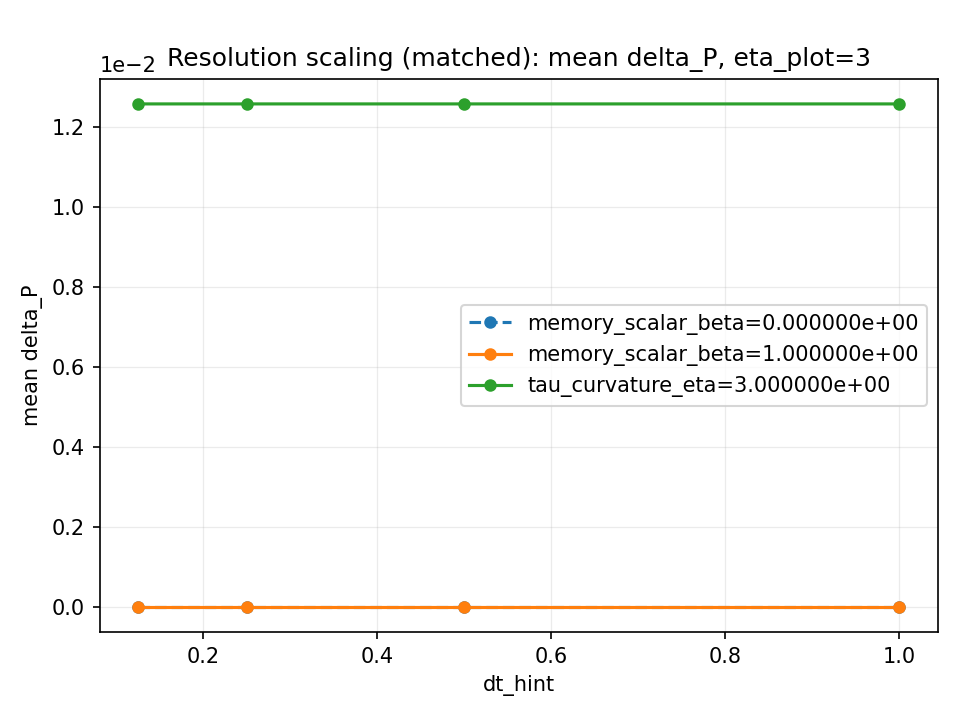
\includegraphics[width=\linewidth]{resolution_scaling_deltaP.png}
  \caption{Resolution scaling of matched-endpoint $\Delta P$.}
\end{subfigure}
\hfill
\begin{subfigure}[t]{0.47\linewidth}
  \centering
  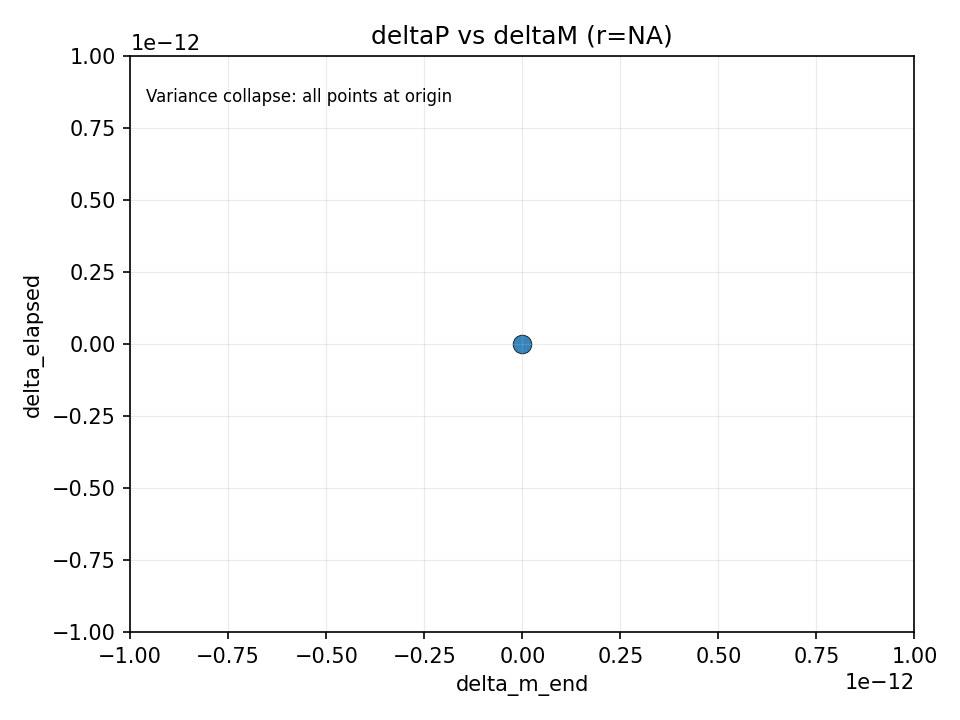
\includegraphics[width=\linewidth]{deltaP_vs_deltaM_matched_scatter.png}
  \caption{Matched-endpoint $\Delta P$ vs $\Delta m$.}
\end{subfigure}

\vspace{0.35em}

\begin{subfigure}[t]{0.47\linewidth}
  \centering
  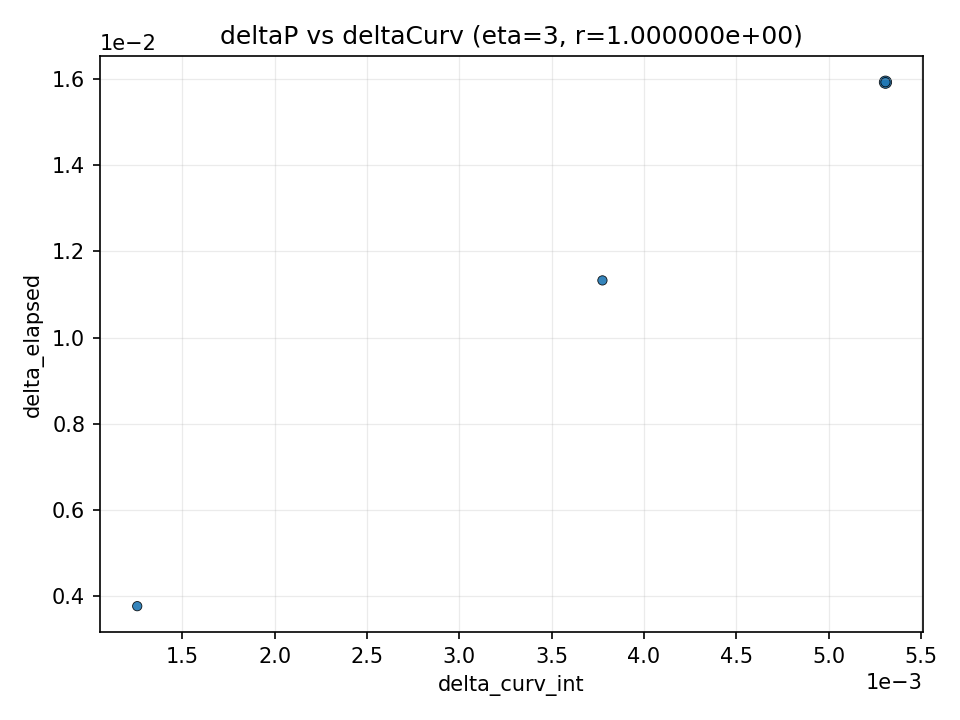
\includegraphics[width=\linewidth]{deltaP_vs_deltaCurv_scatter.png}
  \caption{$\Delta P$ vs $\Delta\kappa$ at $\eta_{\mathrm{plot}}$.}
\end{subfigure}
\hfill
\begin{subfigure}[t]{0.47\linewidth}
  \centering
  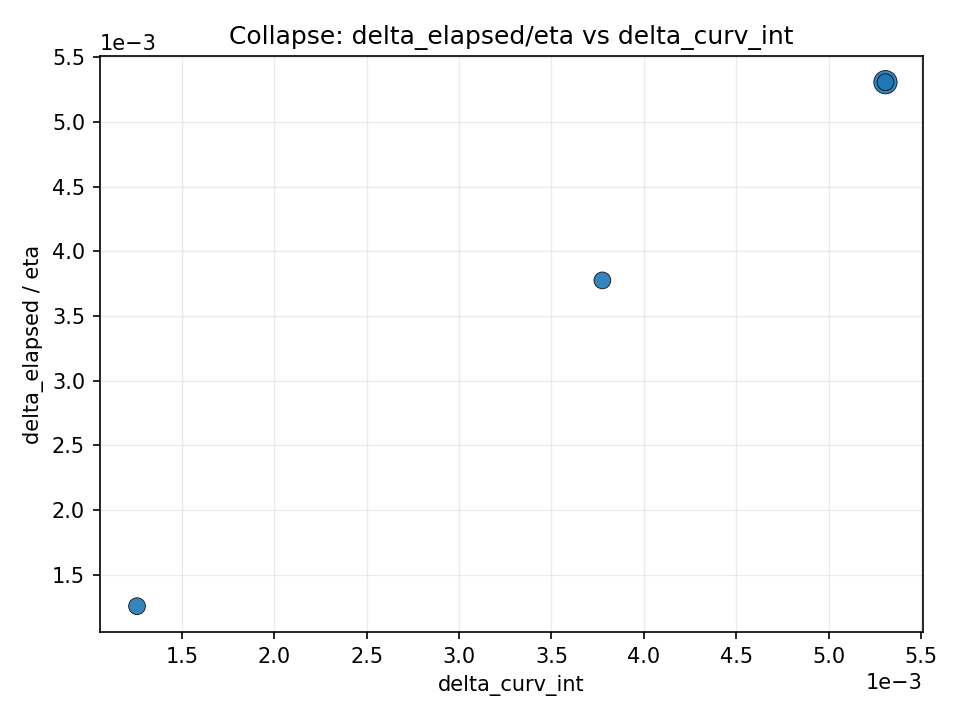
\includegraphics[width=\linewidth]{deltaP_over_eta_vs_deltaCurv_collapse.png}
  \caption{Collapse $\Delta P/\eta$ vs $\Delta\kappa$ across $\eta>0$.}
\end{subfigure}
\caption{Core diagnostics: scaling, endpoint-state relation, and curvature-response collapse.}
\label{fig:core_composite}
\end{figure}

\begin{figure}[t]
\centering
\begin{subfigure}[t]{0.31\linewidth}
  \centering
  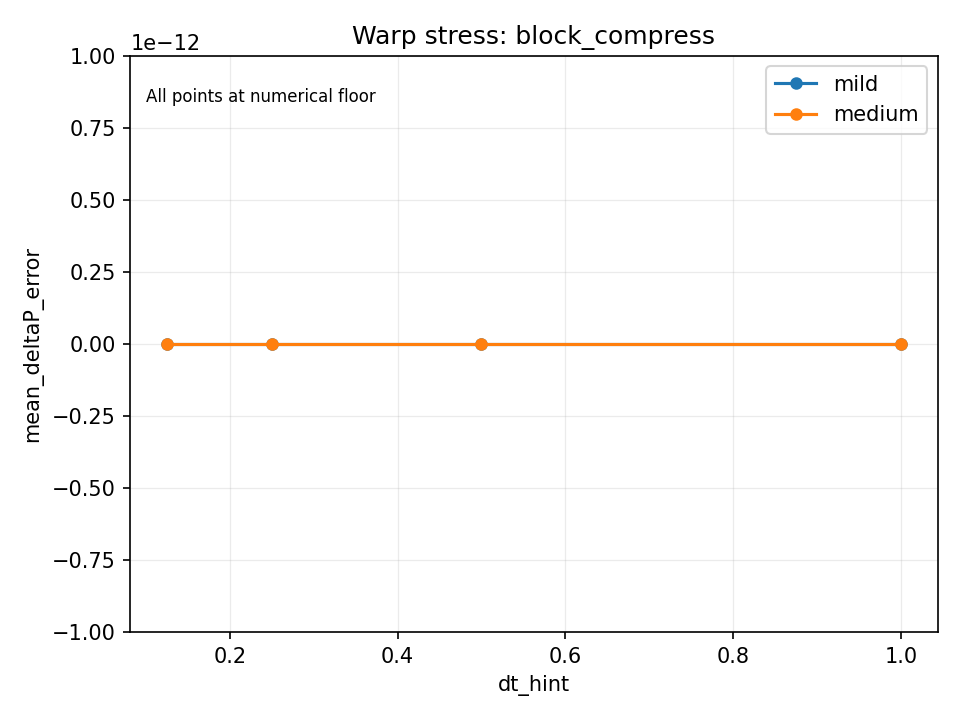
\includegraphics[width=\linewidth]{warp_stress_error_block_compress.png}
  \caption{block\_compress}
\end{subfigure}
\hfill
\begin{subfigure}[t]{0.31\linewidth}
  \centering
  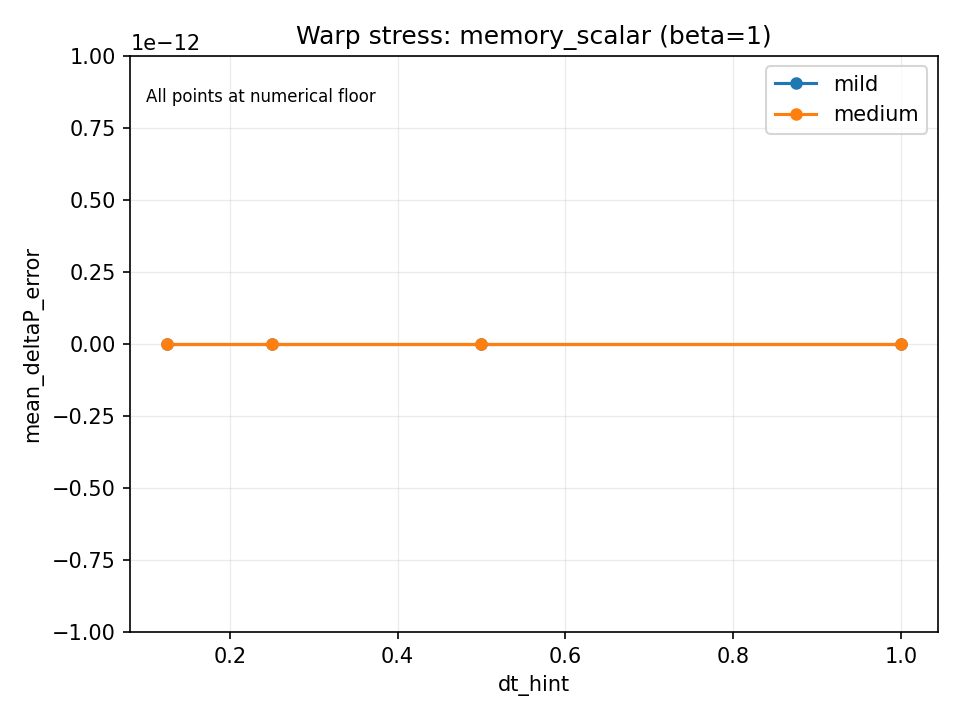
\includegraphics[width=\linewidth]{warp_stress_error_memory_scalar.png}
  \caption{invariant leaky}
\end{subfigure}
\hfill
\begin{subfigure}[t]{0.31\linewidth}
  \centering
  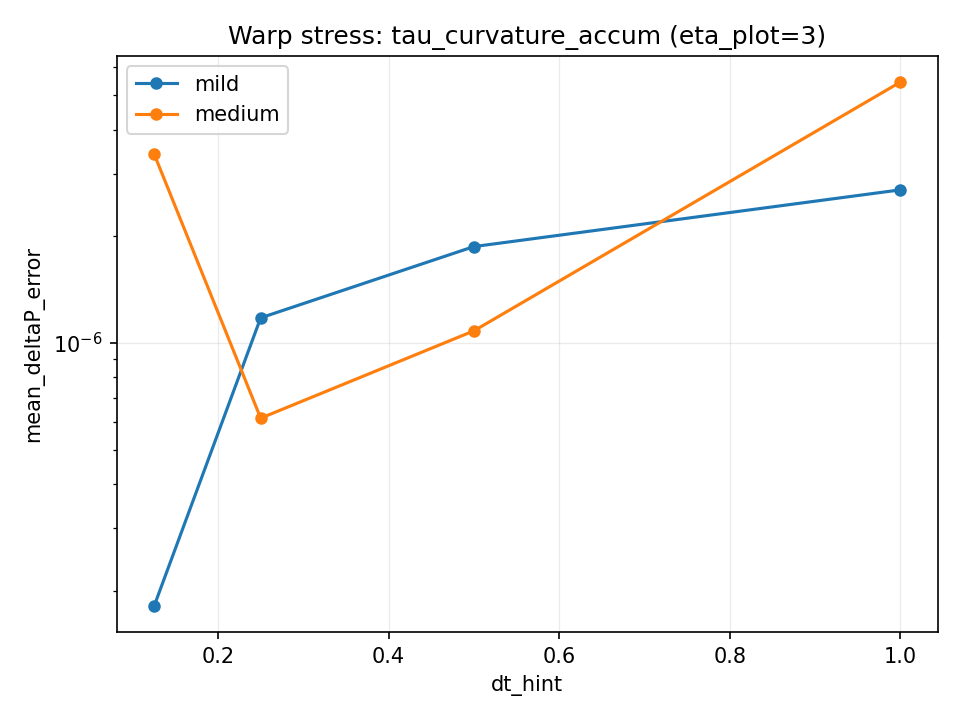
\includegraphics[width=\linewidth]{warp_stress_error_tau_curvature_accum.png}
  \caption{tau\_curvature\_accum}
\end{subfigure}
\caption{Warp-stress comparison across representative model classes.}
\label{fig:gauge_composite}
\end{figure}

\begin{figure}[t]
\centering
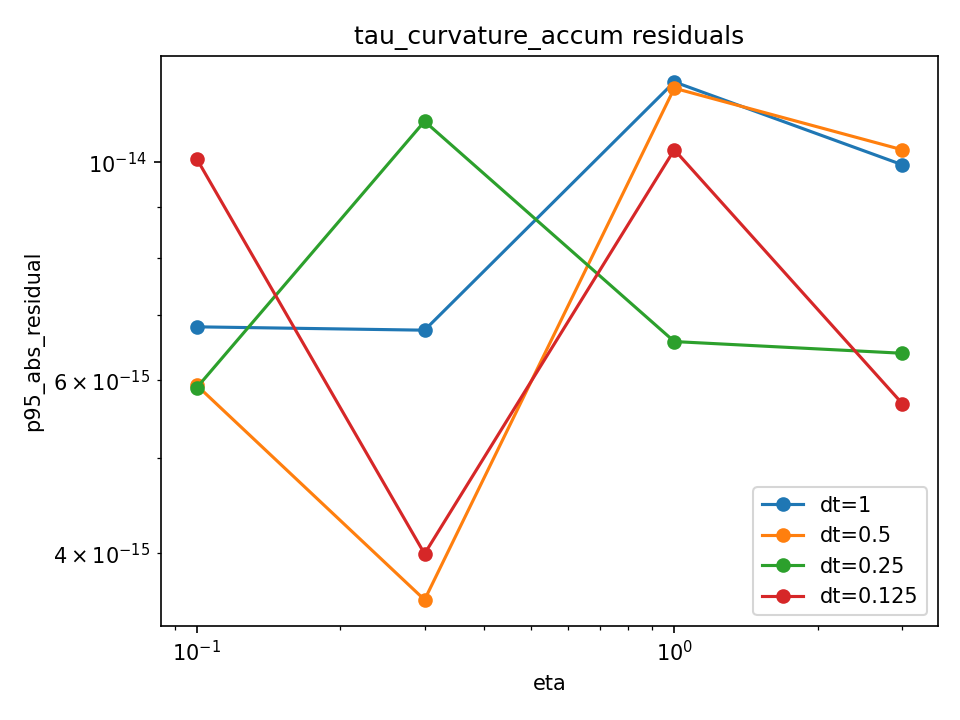
\includegraphics[width=0.56\linewidth]{tau_curv_residuals_vs_eta.png}
\caption{Residual magnitude versus $\eta$ for the curvature-driven fit summary.}
\label{fig:residual_eta}
\end{figure}

The $\tau$-curvature model predicts $\Delta P$ with maximum absolute residual $1.24e\text{-}14$ and maximum relative residual $5.66e\text{-}12$ at $\eta=1.0$ (max over $\Delta t$ resolutions). The fit quality is effectively exact, with $R^2(\Delta P\sim\Delta\kappa)\ge 1.000000$ for $\eta>0$.

\begin{table}[t]
\centering
\caption{Residual summary used in the curvature-fit panel.}
\begin{tabular}{lccccc}
\toprule
$\eta$ & $r(\Delta\kappa,\Delta P)$ & $r(\Delta m,\Delta P)$ & $r(\Delta m,\Delta P\mid\Delta\kappa)$ & max $|\varepsilon|$ & max $|\varepsilon|/|\Delta P|$ \\
\midrule
0.1 & 1.000000e+00 & 4.030289e-01 & -5.793572e-12 & 1.05e-14 & 3.96e-11 \\
0.3 & 1.000000e+00 & 4.030289e-01 & -1.751549e-12 & 1.10e-14 & 2.90e-11 \\
1 & 1.000000e+00 & 4.030289e-01 & -7.679594e-13 & 1.24e-14 & 5.66e-12 \\
3 & 1.000000e+00 & 4.030289e-01 & -6.387632e-13 & 1.07e-14 & 1.89e-12 \\
\bottomrule
\end{tabular}
\end{table}

\newline

\section{Information-Theoretic Interpretation of Internal State}
\label{sec:information_theory}

\paragraph{Model Taxonomy.}
We use two classes, both with the same locked endpoint readout
\[
\Delta P = k\,[m(\tau_T)-m(\tau_0)].
\]
\begin{itemize}
\item \textbf{Class I (Invariant leaky accumulator / Paper-1):}
\[
\frac{dm}{d\tau}=\beta-\lambda m,\qquad
\Delta P = k\,[m(\tau_T)-m(\tau_0)].
\]
The drive is $\tau$-intrinsic.
\item \textbf{Class II (Coordinate-surprise observer):}
\[
\frac{dm}{d\tau}=\beta I(\tau)-\lambda m,\qquad
I(\tau)=\left|\frac{d\log(dt/d\tau)}{d\tau}\right|,\qquad
\Delta P = k\,[m(\tau_T)-m(\tau_0)].
\]
Only the drive differs from Class I.
\end{itemize}

\paragraph{Proposition (Generic coordinate dependence of $I(\tau)$).}
Let $t\mapsto s(t)$ be a strictly monotone reparameterization of coordinate time. Then $r(\tau)$ transforms as
\begin{equation}
r(\tau)\mapsto r_s(\tau)=\frac{ds}{d\tau}=\frac{ds}{dt}\frac{dt}{d\tau}=\frac{ds}{dt}\,r(\tau).
\label{eq:r_transform}
\end{equation}
Hence
\begin{equation}
\frac{d\log r_s}{d\tau}
=
\frac{d\log r}{d\tau}
+
\frac{d}{d\tau}\log\!\left(\frac{ds}{dt}\right),
\label{eq:logr_transform}
\end{equation}
so $I(\tau)=|d\log r/d\tau|$ is not invariant in general (except special cases such as affine $s$).

\paragraph{Proof sketch.}
Equation~\eqref{eq:r_transform} is the chain rule. Taking $\tau$-derivatives of logarithms gives Eq.~\eqref{eq:logr_transform}. The extra additive term is generically nonzero for nonlinear $s(t)$, therefore $I(\tau)$ and any model driven by it are coordinate dependent.
Exception: if $r(\tau)$ is constant along the trajectory family, then $I(\tau)\equiv 0$ and the coordinate-dependent drive term vanishes.

\paragraph{Consequence for matched-endpoint comparisons.}
For matched endpoints $(\tau_0,\tau_T)$, Class I remains invariant up to numerical precision in warp tests, while Class II and fixed-$t$ observers (H1/H2) exhibit finite gauge violation.
Gauge invariance is guaranteed only for $\tau$-intrinsic drives; coordinate-time drives may be invariant on special families ($r$ constant) but are not invariant generically.


\subsection{Leaky-Phase Analysis Under the Locked Invariant Class}
\label{sec:leaky_phase_analysis}

We analyze the Paper-1 invariant class
\[
\frac{dm}{d\tau}=\beta-\lambda m,\qquad
\Delta P = k\,[m(\tau_T)-m(\tau_0)].
\]
The decay parameter $\lambda$ controls the relaxation rate of $m(\tau)$ but cannot create matched-endpoint splitting under constant $\tau$-intrinsic drive; it only attenuates splitting already induced by nontrivial $\tau$-intrinsic inputs.
For fixed endpoints $(\tau_0,\tau_T)$ and fixed initial condition, $\Delta P$ is endpoint-determined; matched-endpoint path pairs therefore do not split under this class.

\paragraph{Numerical phase behavior (\texttt{paper\_final\_20260302}).}
From \texttt{tables/leaky\_memory\_grid.csv} (rows with $\beta=1$, $\mathrm{dt\_hint}=0.5$), terminal memory decreases monotonically with $\lambda$:
\[
m_{\text{end}}(10^{-4})=4256.584,\;
m_{\text{end}}(10^{-3})=996.1074,\;
m_{\text{end}}(10^{-2})=100,\;
m_{\text{end}}(10^{-1})=10,\;
m_{\text{end}}(1)=1.
\]
The matched-path endpoint difference remains numerically zero across the tested grid:
\[
\Delta m_{\text{end}}=0,\qquad \Delta P_{\text{path}}=0.
\]

\paragraph{Interpretation.}
The leaky parameter $\lambda$ controls memory amplitude and horizon, not gauge violation. In this locked invariant class:
\begin{itemize}
\item $\lambda$ modulates endpoint state magnitude $m(\tau_T)$.
\item matched-endpoint path comparisons remain collapsed ($\Delta P_{\text{path}}=0$).
\item gauge separation must therefore be established against coordinate-dependent observers (Section~\ref{sec:model_class_comparison}).
\end{itemize}


\subsection{Model-Class Gauge Comparison}
\label{sec:model_class_comparison}

We compare one invariant class and three coordinate-dependent observers:
\[
\text{Invariant:}\quad
\frac{dm}{d\tau}=\beta-\lambda m,\quad
\Delta P = k\,[m(\tau_T)-m(\tau_0)].
\]
\[
\text{Coordinate surprise:}\quad
\frac{dm}{d\tau}=\beta I(\tau)-\lambda m,\quad
I(\tau)=\left|\frac{d\log(dt/d\tau)}{d\tau}\right|,\quad
\Delta P = k\,[m(\tau_T)-m(\tau_0)].
\]
\[
H_1(t)=|\dot\tau(t)-1|,\quad P_{H_1}=\int H_1(t)\,dt,\qquad
H_2(t)=|\ddot\tau(t)|,\quad P_{H_2}=\int H_2(t)\,dt.
\]

\paragraph{Warp metric and gate policy.}
For each model we compute
\[
\Delta P_{\text{warp}}=|P(\tau)-P(\tau\circ s)|.
\]
Family A ($\tau=t$) is sanity-only; Family B ($\tau=T(t/T)^{1.2}$) is the separation gate.
Ratios use the reported floor denominator from the same run:
\[
\mathrm{ratio}=\frac{\max\_error}{\max(\max\_error_{\text{inv}},\epsilon_{\text{floor}})}.
\]

\begin{figure}[H]
\centering
\begin{subfigure}[t]{0.49\linewidth}
  \centering
  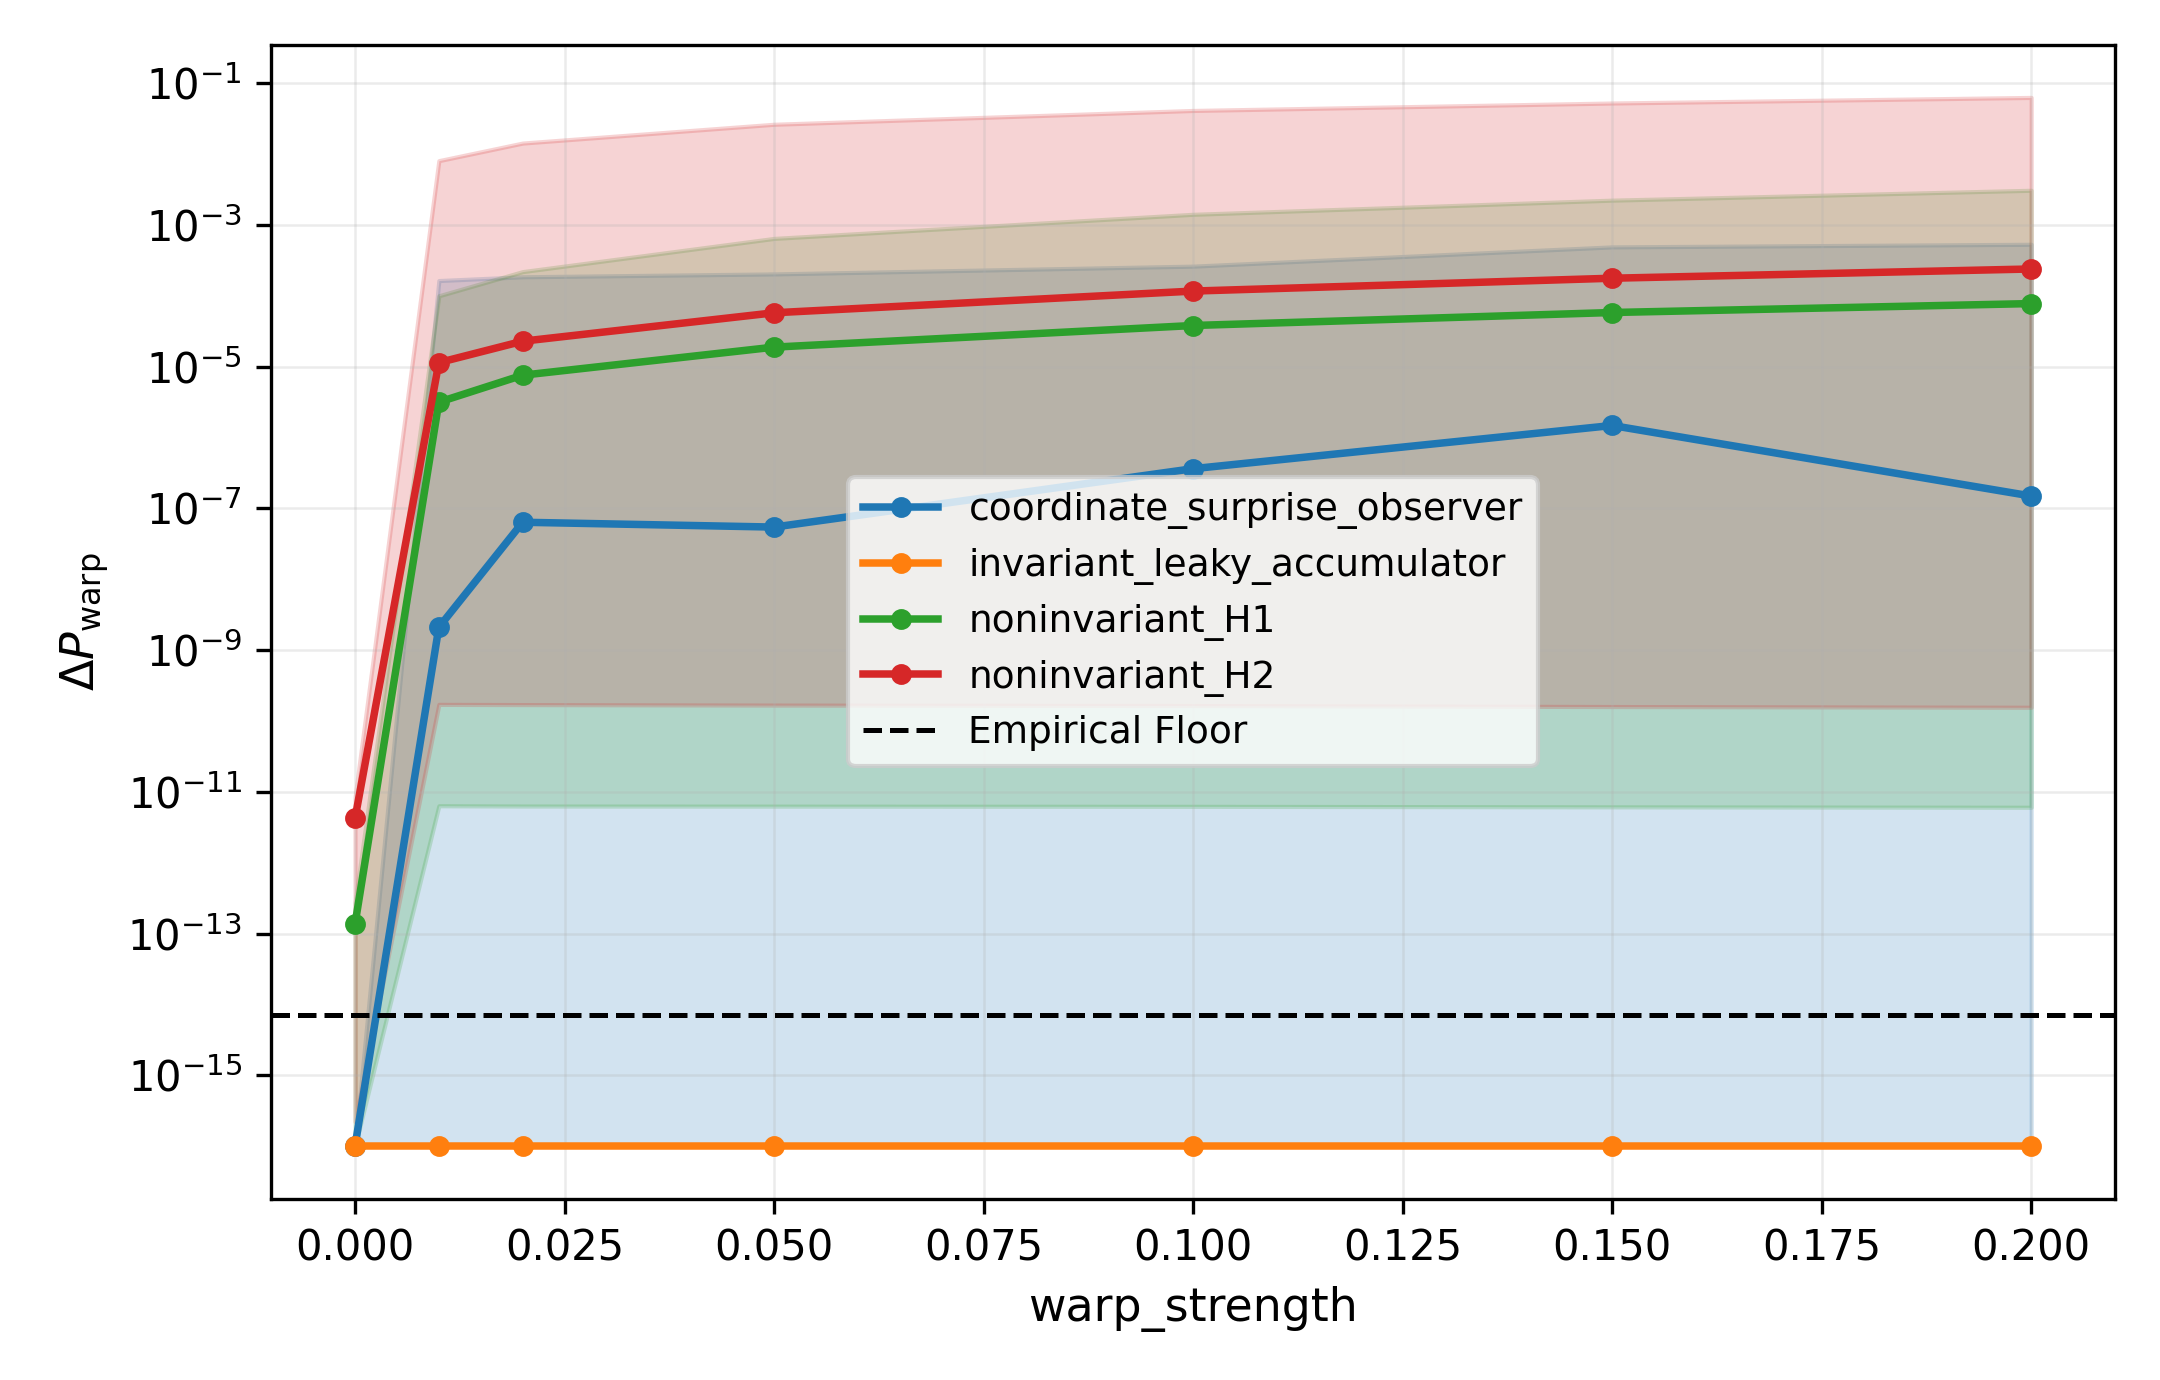
\includegraphics[width=\linewidth]{plots/main_fig1_warp_sweep.png}
  \caption{Warp-strength sweep using per-warp samples (median with p5--p95 band).}
\end{subfigure}
\hfill
\begin{subfigure}[t]{0.49\linewidth}
  \centering
  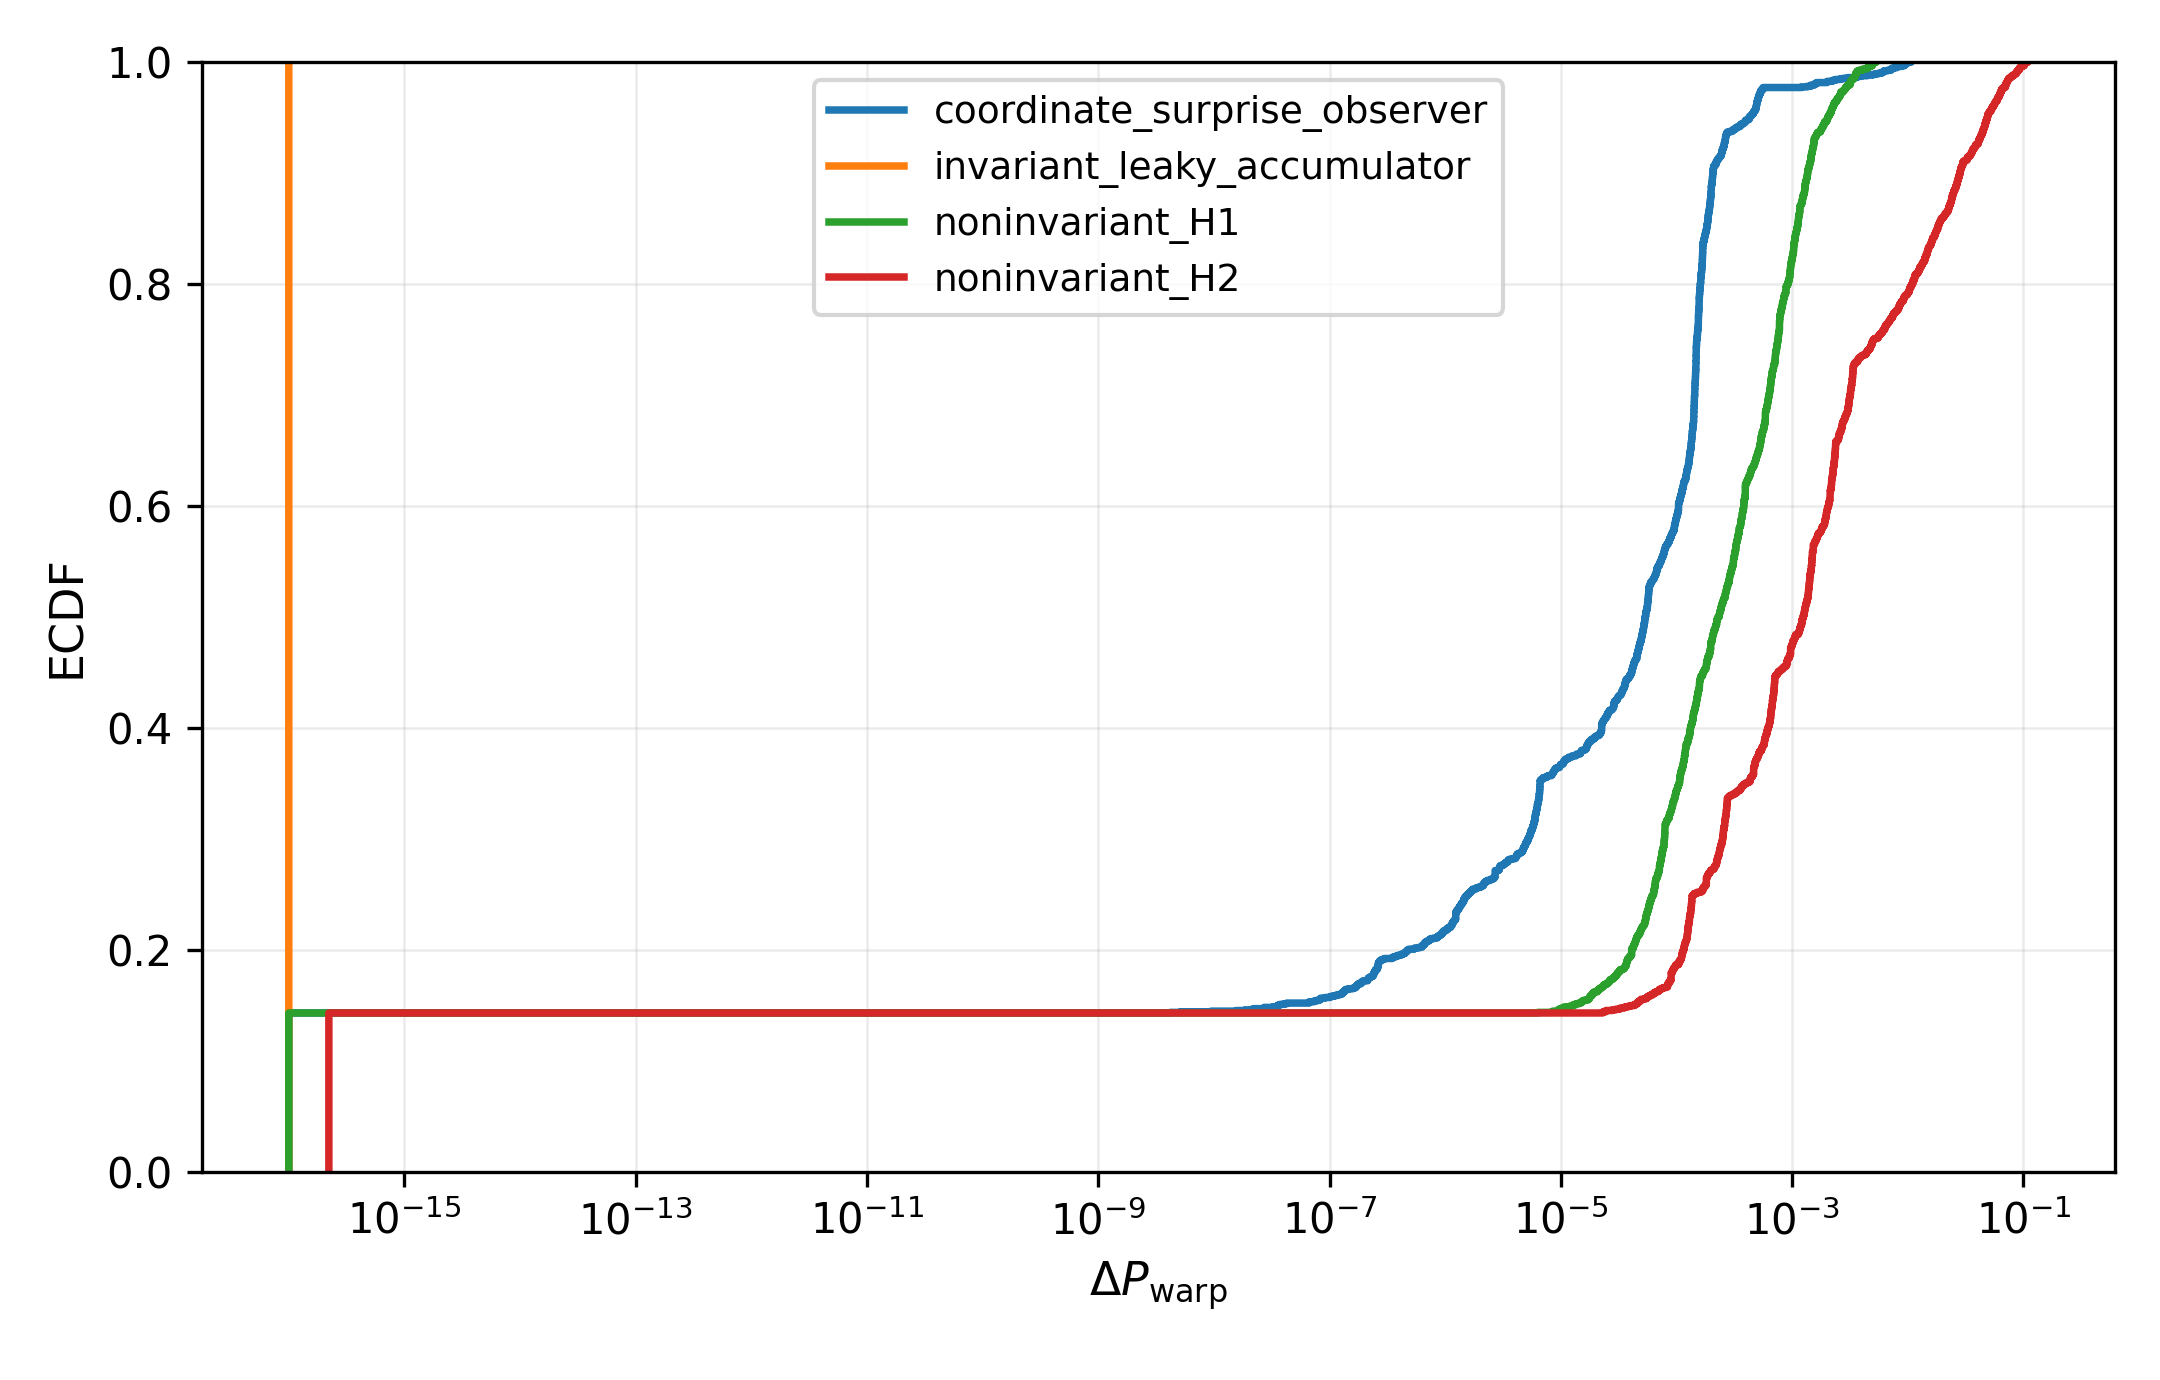
\includegraphics[width=\linewidth]{plots/main_fig2_ecdf_familyB.png}
  \caption{Family-B ECDF of $\Delta P_{\mathrm{warp}}$ by model class.}
\end{subfigure}
\caption{Main gauge-comparison figures generated from \texttt{per\_warp\_results.csv} and \texttt{gauge\_violation\_comparison.csv}.}
\label{fig:main_gauge_figures}
\end{figure}

\paragraph{Final separation (\texttt{paper\_final\_20260302}, Family B).}
Using \texttt{tables/gauge\_violation\_comparison.csv}:
\begin{table}[H]
\centering
\caption{Family-B gauge-violation separation using
\[
\mathrm{ratio\_to\_invariant}
=
\frac{\mathrm{max\_error}}{\epsilon_{\mathrm{floor,used}}},
\qquad
\epsilon_{\mathrm{floor,used}}=\max(\mathrm{EPS\_FLOOR},\epsilon_{\mathrm{floor,empirical}}).
\]
The invariant baseline is reported as $\mathrm{max\_error}=0$ (within floor) and ratio $=1.0$.}
\label{tab:gauge_violation_final_B}
\begin{tabular}{@{}lcc@{}}
\toprule
Model & max\_error & ratio\_to\_invariant \\
\midrule
Invariant leaky accumulator & 0 & 1.0 \\
Coordinate-surprise observer & $2.574388685956\times 10^{-2}$ & $3.660237056255\times 10^{12}$ \\
H1 & $3.619835733440\times 10^{-2}$ & $5.146641981986\times 10^{12}$ \\
H2 & $2.134064697311\times 10^{-1}$ & $3.034189331298\times 10^{13}$ \\
\bottomrule
\end{tabular}
\end{table}

All noninvariant observers pass the separation gate ($\ge 10^6$) by multiple orders of magnitude, while the invariant class remains at numerical floor.


The experimental figures and tables show three core findings. First, memoryless gauge-invariant models exhibit endpoint collapse: matched-endpoint trajectories yield identical perceived duration, and this holds under resolution refinement and strong reparameterizations. Second, the locked invariant memory baseline with constant drive remains endpoint-collapsed for matched-endpoint comparisons. Third, invariant interior sensitivity is recovered only when the drive is nontrivial in $\tau$-space (curvature/event-like signal), while coordinate-dependent observers fail gauge consistency by orders of magnitude.

Resolution scaling and warp stress tests confirm the invariant baseline and the class separation. The controlled-break plots show endpoint collapse in memoryless and constant-drive invariant baselines, while nontrivial $\tau$-intrinsic drives produce the matched-endpoint split without violating invariance. Curvature-extension plots quantify this nontrivial-drive regime.

\section{Discussion}

Our findings imply that changes in perceived time with age cannot arise from coordinate-time derivative effects alone. Within the invariant framework, memory is necessary but not sufficient for matched-endpoint splitting: a nontrivial $\tau$-intrinsic drive is additionally required. The model comparison (Section~\ref{sec:model_class_comparison}) demonstrates that invariant and coordinate-dependent classes are decisively separated, confirming gauge invariance as a structural requirement rather than a convenience.

The framework naturally opens the door to entropy-based interpretations, surprise accumulation, and links to Weber--Fechner-like laws without sacrificing invariance principles.

\section{Conclusion}

We have shown that:
\begin{itemize}
\item Reparameterization invariance enforces endpoint collapse in memoryless models.
\item Time derivatives alone are insufficient to alter perception.
\item Internal memory is necessary but not sufficient for matched-endpoint interior sensitivity in the invariant class.
\item Matched-endpoint splitting requires a nontrivial $\tau$-intrinsic drive while preserving the locked endpoint readout.
\end{itemize}

This establishes a principled taxonomy for modeling subjective time that is mathematically consistent with gauge constraints and matched-endpoint tests.

\bigskip
\newpage
\bibliographystyle{unsrt}
\bibliography{references}


\end{document}
